% Created 2021-02-19 Fri 14:31
% Intended LaTeX compiler: pdflatex
\documentclass[11pt]{article}
\usepackage[utf8]{inputenc}
\usepackage[T1]{fontenc}
\usepackage{graphicx}
\usepackage{grffile}
\usepackage{longtable}
\usepackage{wrapfig}
\usepackage{rotating}
\usepackage[normalem]{ulem}
\usepackage{amsmath}
\usepackage{textcomp}
\usepackage{amssymb}
\usepackage{capt-of}
\usepackage{hyperref}
\usepackage{amsthm}
\usepackage{url}
\usepackage[margin=.5in]{geometry}
\usepackage{hyperref}
\usepackage[dvipsnames]{xcolor}
\usepackage{booktabs}
\usepackage{enumitem}
\newtheorem*{definition}{Definition}
\newtheorem*{example}{Example}
\newtheorem*{theorem}{Theorem}
\newtheorem*{corollary}{Corollary}
\newtheorem*{exercise}{Exercise}
\newtheorem*{problem}{Problem}
\newtheorem{question}{Question}
\newcommand{\gr}{\textcolor{ForestGreen}}
\newcommand{\rd}{\textcolor{red}}
\newcommand{\R}{\mathbb{R}}
\newcommand{\p}{\mathbb{P}}
\newcommand{\E}{\mathbb{E}}
\newcommand{\frall}{\ \forall}
\newcommand{\st}{_{s_t}}
\newcommand{\var}{\operatorname{Var}}
\newcommand{\cov}{\operatorname{Cov}}
\newcommand{\cor}{\operatorname{Cor}}
\author{Chris Ackerman\thanks{I worked on this problem set with Ekaterina Gurkova, Luna Shen, Ben Pirie and Ali Haider Ismail.}}
\date{\today}
\title{Econ202B HW4}
\hypersetup{
 pdfauthor={Chris Ackerman\thanks{I worked on this problem set with Ekaterina Gurkova, Luna Shen, Ben Pirie and Ali Haider Ismail.}},
 pdftitle={Econ202B HW4},
 pdfkeywords={},
 pdfsubject={},
 pdfcreator={Emacs 28.0.50 (Org mode 9.3)}, 
 pdflang={English}}
\begin{document}

\maketitle
\tableofcontents

\newpage

\section{Question 1}
\label{sec:org921e40e}
\begin{enumerate}[label=\alph*)]
\item Each generation faces the same problem, except the initial old, since they don't have any problem when they're young.
\begin{align*}
\max c_{i1}^o \tag{initial old}\\
\text{s.t.\quad } c_{i1}^o &= y_{i1}^o + q_0 m_i \tag{initial old}\\
\max u_i(c_{it}^y, c_{it+1}^o) \tag{other generations}\\
s.t. p_t c_{it}^y + p_{t +  1}c_{it+1}^o &= p_t y_{it}^y + p_{t + 1} y_{it+1}^o \tag{other generations}\\
\intertext{Feasibility in period $t$ requires}
c_{1t}^y + c_{2t}^y    c_{1t}^o + c_{2t}^o &= y_{1t}^y + y_{2t}^y    y_{1t}^o + y_{2t}^o
\end{align*}
A competitive equilibrium consists of
\begin{enumerate}
\item An allocation for the initial old, $(c_{11}^o, c_{12}^o)$
\item Money holdings for the initial old, $(m_1, m_2)$
\item Allocations for each generation $t$, $\left\{c_{1t}^y, c_{2t}^y, c_{1t+1}^o, c_{2t+1}^o\right\}^\infty_{t = 1}$
\item An initial price of money $q_0$
\item Prices for consumption $\left\{p_t\right\}^\infty_{t = 1}$
\end{enumerate}
such that, given prices and endowments the allocations solve each agent's maximization problem and are feasible, for each time period.

\item
From our definition of equilibrium, each agent's consumption must maximize their utility. Since utility (should be) strictly increasing in young consumption and old consumption, each agent's budget constraint should hold with equality,
\[
p_t c_{it}^y + p_{t+1}c_{it+1}^o = p_t y_{it}^y + p_{t + 1}c_{it + 1}^o, \quad i \in \{1, 2\}.
\]
We want to show
\[
p_t (c_{1t}^y c_{2t}^y) + p_{t+1}(c_{1t+1}^o c_{2t+1}^o) = p_t (y_{1t}^y y_{2t}^y) + p_{t + 1}(c_{1t + 1}^o + c_{2t + 1}^o),
\]
which follows from summing the budget constraint across agents.

\item
The FOC for utility maximization gives
\[
\frac{du_i(c_{it}^y, c_{it+1}^o/dc_{it}^y}{du_i(c_{it}^y, c_{it+1}^o)/dc_{it + 1}^o} = \frac{p_t}{p_{t + 1}}.
\]
Since both agents face the same prices, it must be that 
\[
\frac{du_1(c_{1t}^y, c_{1t+1}^o/dc_{1t}^y}{du_1(c_{1t}^y, c_{1t+1}^o)/dc_{1t + 1}^o} =\frac{du_2(c_{2t}^y, c_{2t+1}^o/dc_{2t}^y}{du_2(c_{2t}^y, c_{2t+1}^o)/dc_{2t + 1}^o}.
\]
Given different utility functions and endowments, this relationship will only hold in very special cases, so we should expect to see trade within generations given this setup.

\item
Let's construct an equilibrium that satisfies these criteria. Start with \(q_0 m = 0\) so that the initial old can't trade. Then the initial old just consume their endowments. From the requirement that the young consume their entire endowment, we have
\[
c_1^y + c_2^y = y_1^y + y_2^y.
\]
Utility maximization gives
\[
\frac{du_1(c_{1t}^y, c_{1t+1}^o/dc_{1t}^y}{du_1(c_{1t}^y, c_{1t+1}^o)/dc_{1t + 1}^o} =\frac{du_2(c_{2t}^y, c_{2t+1}^o/dc_{2t}^y}{du_2(c_{2t}^y, c_{2t+1}^o)/dc_{2t + 1}^o} = R,
\]
and the intertemporal budget constraint gives
\[
c_i^y + \frac{c_i^o}{R} = y_i^y + \frac{y_i^o}{R}.
\]
We now have five independent equations in five unknowns, so we can normalize \(p_1\) and use \(R = p_t / p_{t+1}\) to construct an equilibrium price vector.

\item
We want to check equilibria with no trade, with some trade, and unstable equilibria. For autarky, we need
\begin{align*}
q_0(m_1 + m_2) &= 0,\\
c_{i1}^o &= y_{i1}^0, \quad i \in \{1, 2\}\\
\frac{\alpha c_1^o}{c^y_1} &= R \tag{type 1 FOC}\\
c^y_1 + \frac{c^o_1}{R} &= y^y_1 + \frac{y^o_1}{R}\tag{budget constraint}\\
c_1^y &= \frac{\alpha}{1  + \alpha} (y_1^y + y_1^o/R)\\
c^o_1 &= \frac{1}{1 + \alpha} (Ry^y_1 + y^o_1)\\
\intertext{For agent 2 \ldots }
c_2^y &= \frac{1}{1  + \alpha} (y_2^y + y_2^o/R)\\
c^o_2 &= \frac{\alpha}{1 + \alpha} (Ry^y_2 + y^o_2)\\
\intertext{If the young aren't trading with the old, we have}
c^y_1 + c^y_2 &= y^y_1 + y^y_2\\
\implies R = \frac{\alpha y^o_1 + y^o_2}{y^y_1 + y^y_2} &= \frac{\alpha + 2}{3 + 2 \alpha}
\end{align*}
This \(R < 1\) supports a stationary equilibrium without trade across generations for any \(\alpha \in [0, 1]\). Now let's check for an equilibrium with trade and \(R = 1\). We'll start with the demand functions, 
\begin{align*}
c_1^y &= \frac{\alpha}{1  + \alpha} (y_1^y + y_1^o)\\
c^o_1 &= \frac{1}{1 + \alpha} (y^y_1 + y^o_1)\\
c_2^y &= \frac{1}{1  + \alpha} (y_2^y + y_2^o)\\
c^o_2 &= \frac{\alpha}{1 + \alpha} (y^y_2 + y^o_2)\\
\intertext{The feasibility condition with trade is}
c_1^y + c_2^y +c_1^o + c_2^o &= y_1^y + y_2^y + y_1^o + y_2^o\\
\intertext{Now we need to give the initial old enough money to pay for the trade they want:}
q_0 (m_1 + m_2) &= (y_1^o + y_2^o) - (c_1^o - c_2^o).
\end{align*}
There are also non-stationary equilibria with
\[
q_o (m_1 + m_2) \in [0, (y_1^o + y_2^o) - (c_1^o + c_2^o)].
\]
\end{enumerate}

\section{Question 2}
\label{sec:org3d38114}
\begin{enumerate}
\item \begin{center}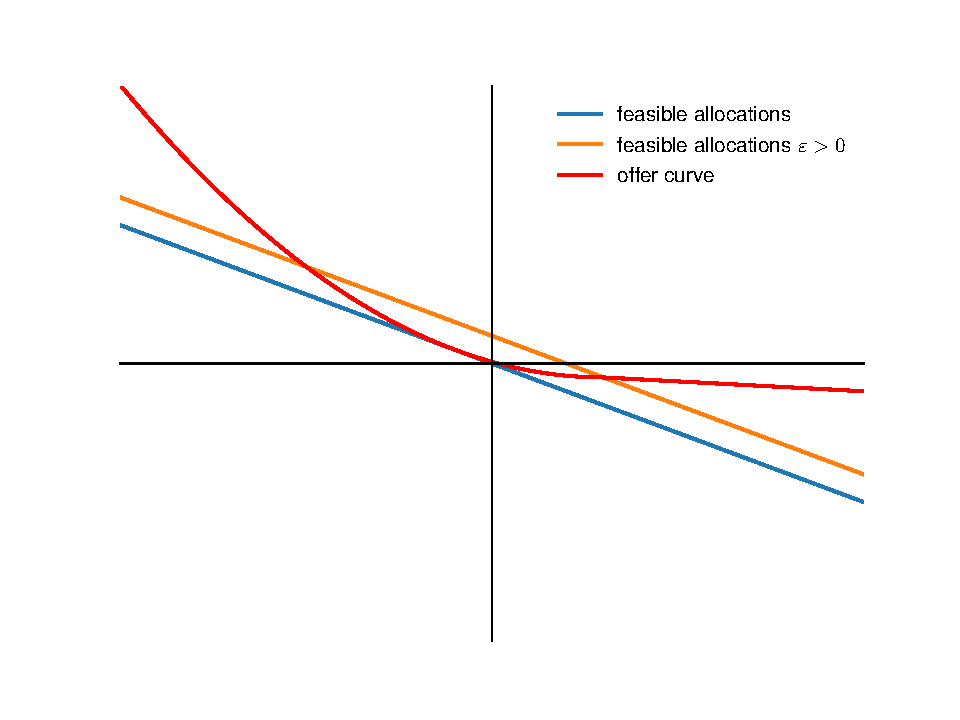
\includegraphics[width=\textwidth, keepaspectratio=true]{offer_curve.pdf}\end{center}
\item 
This setup shifts the feasibility line out, so the initial equilibrium at the origin is not an equilibrium anymore. The unique stationary equilibrium is now the one associated with $R > 1$.
\item
\begin{align*}
R &= \frac{y^o + \varepsilon}{y^y}\\
&= \frac{1 + \varepsilon}{3}
\end{align*}
For $\varepsilon$ small, $R < 1$. The young want to save, so $q_T \in [0, 1]$, and the budget constraint when $R = 1$ is
\begin{align*}
c_T^o &= y^y + y^o - c^y_T \\
&= 2
\end{align*}
which requires $q_T = 1$.


When $\varepsilon > 2$,
\[
\frac{1 + \varepsilon}{3} > 1,
\]
autarky is the unique satable equilibrium, and $q_T = 0$.
\end{enumerate}

\section{Question 3}
\label{sec:org6ad3cf1}
  \begin{enumerate}[label=\alph*)]
\item
  \begin{align*}
\max c_1^o \quad &\text{ s.t. } c_1^o = 1 + q_0 m \tag{initial old}\\
\max &u(c_t^y, c_{t + 1}^o) \tag{other generations}\\
\text{s.t. } \quad c^y_t + \frac{1}{R_t} c^o_{t + 1} &= (y^y - \tau_t) + \frac{1}{R_t}y^o\\
&= 2 + \frac{1}{R_t}\\
g_t &= \tau_t \tag{government}\\
c_t^y + c_t^o + g &= y^y + y^o \tag{feasibility}\\
&= 3 + 1
  \end{align*}
A competitive equilibrium is
\begin{enumerate}
\item An allocation for the initial old
\item Allocations for each generation, $\{c^y_t, c^o_{t + 1}\}^\infty_{t = 1}$
\item Interest rates $\{R_t\}^\infty_{t = 1}$
\item An initial price of money $q_0$
\item Government policies $\{g_t, \tau_t\}^\infty_{t = 1}$
\end{enumerate}
such that the allocations solve agents' problems, and the allocations and government policies satisfy feasibility. Now check if \(R_t = 1\), \(c_t^o = c_t^y = 3/2\) and \(g_t = \tau_t = 1\) for all \(t \ge 1\) satisfy this definition.

First, \(c_t^y = 3/2 \implies q_0 m = 1/2\). The first order conditions for other generations give
\[
\frac{c^o_{t + 1}}{c_t^y} = R_t.
\]
Our proposed consumptions and interest rates satisfy this. Autarky is also a stationary equilibrium and requires \(q_o m = 0\), and there are non-stationary equilibria with \(q_o m \in (0, 1/2)\).

\item Let's start with the young, then the old, and then the government
\begin{align*}
c_1^y &= y^y + y^o - c_1^o - g_1\\
&= 3/2 \\
R &= \frac{u_1(c_1^y, c_2^o)}{u_2(c_1^y, c_2^o)} \tag{FOC}\\
&= \frac{c_2^o}{c_1^y}\\
\implies c_2^o &= 3/2\\
c_2^y &= y^y + y^o - c_2^o - g_2\\
&= 3/2\\
\intertext{$c^g = 3/2 ,g \in \{o, y\}$ holds for all generations.}
B_1 = g_1 - \tau_1 \\
&= 3/2 - 1\\
&= 1/2 
\end{align*}
The government will never pay down the principly on its debt, but simply keep this balance of \(1/2\) forever.

\item Set \(g_1 = 3/2 + \varepsilon\) and start checking the conditions for equilibria.

\begin{align*}
c_1^y &= y^y + y^o - g_1 - c_1^o \\
&= 3 + 1 - (3/2 + \varepsilon) - 1 \\
&= 3/2 - \varepsilon\\
R_1 &= \frac{c_2^o}{c_1^y}\\
&= \frac{c_2^o}{3/2 - \varepsilon}\\
c_1^y + \frac{c_2^o}{R_1} &= 2 + \frac{1}{R_1}\\
R_1 &= \frac{1}{1 - 2 \varepsilon}\\
\implies c_o^2 &= \frac{3 - 2\varepsilon}{2 - 4\varepsilon}\\
\intertext{From feasibility and utility maximization at date 2,}
R_2 &= \frac{c_3^o(2 - 4\varepsilon)}{3 - 10\varepsilon}\\
\implies R_2 &= \frac{1 - 2\varepsilon}{1 - 6 \varepsilon}
\end{align*}
Thus the interest rate increases each period, so it is not an equilibrium to have \(g_1 > 3/2\), then \(g_t = 1 \forall t \ge 2\) with \(\tau_t = 1\).
  \end{enumerate}
\end{document}